\documentclass[tikz, border=10pt]{standalone}
\usepackage{tikz}
\usepackage[sfdefault]{ClearSans}
\usepackage[T1]{fontenc}
\usetikzlibrary{shapes.misc, positioning, arrows.meta, fit, calc}

\begin{document}

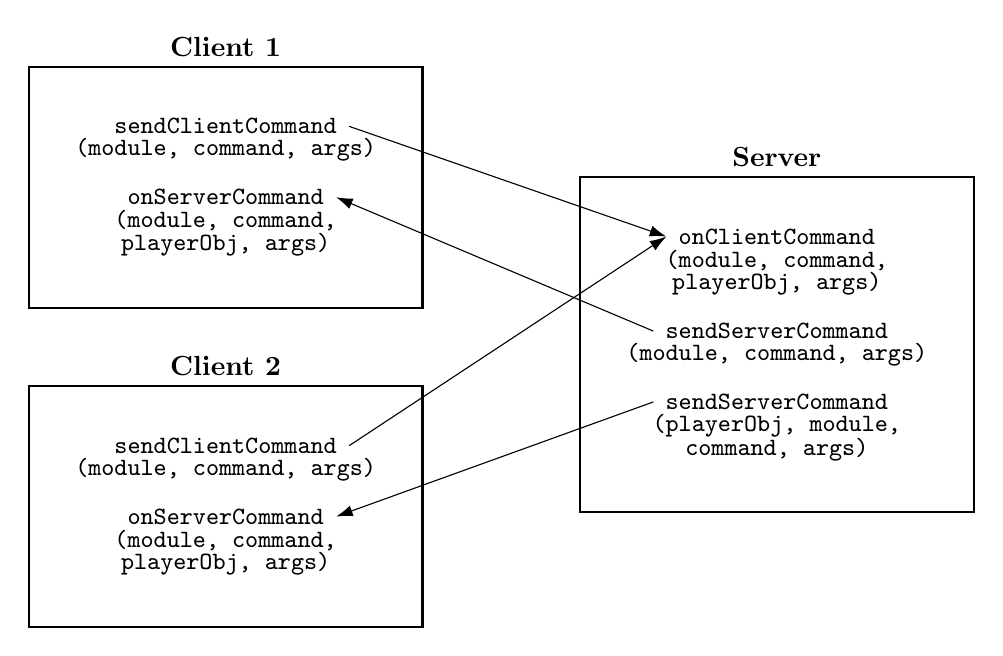
\begin{tikzpicture}[
    node distance=0.3cm,
    box/.style={rectangle, draw, thick, minimum width=5cm, inner sep=0.5cm},
    func/.style={font=\ttfamily\small, inner sep=0.15cm},
]

    % Client 1 functions
    \node[func] (c1_send) {sendClientCommand};
    \node[func, below of=c1_send] (c1_send_args) {(module, command, args)};
    \node[func, below of=c1_send_args] (c1_space1) {};
    \node[func, below of=c1_space1] (c1_recv) {onServerCommand};
    \node[func, below of=c1_recv] (c1_recv_args) {(module, command,};
    \node[func, below of=c1_recv_args] (c1_recv_args2) {playerObj, args)};

    % Create bounding box for Client 1
    \node[box, fit=(c1_send) (c1_recv_args2), label={above:\textbf{Client 1}}] (client1_box) {};

    % Client 2 functions
    \node[func, below=2cm of c1_recv_args2] (c2_send) {sendClientCommand};
    \node[func, below of=c2_send] (c2_send_args) {(module, command, args)};
    \node[func, below of=c2_send_args] (c2_space1) {};
    \node[func, below of=c2_space1] (c2_recv) {onServerCommand};
    \node[func, below of=c2_recv] (c2_recv_args) {(module, command,};
    \node[func, below of=c2_recv_args] (c2_recv_args2) {playerObj, args)};

    % Create bounding box for Client 2
    \node[box, fit=(c2_send) (c2_recv_args2), label={above:\textbf{Client 2}}] (client2_box) {};

    % Server functions
    \node[func] at ($(c1_send)+(7cm, -1.4cm)$) (s_recv) {onClientCommand};
    \node[func, below of=s_recv] (s_recv_args) {(module, command,};
    \node[func, below of=s_recv_args] (s_recv_args2) {playerObj, args)};
    \node[func, below of=s_recv_args2] (s_space1) {};
    \node[func, below of=s_space1] (s_send1) {sendServerCommand};
    \node[func, below of=s_send1] (s_send1_args) {(module, command, args)};
    \node[func, below of=s_send1_args] (s_space2) {};
    \node[func, below of=s_space2] (s_send2) {sendServerCommand};
    \node[func, below of=s_send2] (s_send2_args) {(playerObj, module,};
    \node[func, below of=s_send2_args] (s_send2_args2) {command, args)};

    % Create bounding box for Server
    \node[box, fit=(s_recv) (s_send2_args2), label={above:\textbf{Server}}] (server_box) {};

    % Draw arrows
    % Client 1 sendClientCommand -> Server onClientCommand
    \draw[-{Latex[length=6pt, width=4pt]}] (c1_send.east) -- (s_recv.west);
    
    % Server sendServerCommand -> Client 1 onServerCommand
    \draw[-{Latex[length=6pt, width=4pt]}] (s_send1.west) -- (c1_recv.east);

    % Client 2 sendClientCommand -> Server onClientCommand
    \draw[-{Latex[length=6pt, width=4pt]}] (c2_send.east) -- (s_recv.west);
    
    % Server sendServerCommand(playerObj, ...) -> Client 2 onServerCommand
    \draw[-{Latex[length=6pt, width=4pt]}] (s_send2.west) -- (c2_recv.east);

\end{tikzpicture}

\end{document}
